% Options for packages loaded elsewhere
\PassOptionsToPackage{unicode}{hyperref}
\PassOptionsToPackage{hyphens}{url}
%
\documentclass[
]{article}
\usepackage{amsmath,amssymb}
\usepackage{lmodern}
\usepackage{iftex}
\ifPDFTeX
  \usepackage[T1]{fontenc}
  \usepackage[utf8]{inputenc}
  \usepackage{textcomp} % provide euro and other symbols
\else % if luatex or xetex
  \usepackage{unicode-math}
  \defaultfontfeatures{Scale=MatchLowercase}
  \defaultfontfeatures[\rmfamily]{Ligatures=TeX,Scale=1}
\fi
% Use upquote if available, for straight quotes in verbatim environments
\IfFileExists{upquote.sty}{\usepackage{upquote}}{}
\IfFileExists{microtype.sty}{% use microtype if available
  \usepackage[]{microtype}
  \UseMicrotypeSet[protrusion]{basicmath} % disable protrusion for tt fonts
}{}
\makeatletter
\@ifundefined{KOMAClassName}{% if non-KOMA class
  \IfFileExists{parskip.sty}{%
    \usepackage{parskip}
  }{% else
    \setlength{\parindent}{0pt}
    \setlength{\parskip}{6pt plus 2pt minus 1pt}}
}{% if KOMA class
  \KOMAoptions{parskip=half}}
\makeatother
\usepackage{xcolor}
\usepackage[margin=1in]{geometry}
\usepackage{color}
\usepackage{fancyvrb}
\newcommand{\VerbBar}{|}
\newcommand{\VERB}{\Verb[commandchars=\\\{\}]}
\DefineVerbatimEnvironment{Highlighting}{Verbatim}{commandchars=\\\{\}}
% Add ',fontsize=\small' for more characters per line
\usepackage{framed}
\definecolor{shadecolor}{RGB}{248,248,248}
\newenvironment{Shaded}{\begin{snugshade}}{\end{snugshade}}
\newcommand{\AlertTok}[1]{\textcolor[rgb]{0.94,0.16,0.16}{#1}}
\newcommand{\AnnotationTok}[1]{\textcolor[rgb]{0.56,0.35,0.01}{\textbf{\textit{#1}}}}
\newcommand{\AttributeTok}[1]{\textcolor[rgb]{0.77,0.63,0.00}{#1}}
\newcommand{\BaseNTok}[1]{\textcolor[rgb]{0.00,0.00,0.81}{#1}}
\newcommand{\BuiltInTok}[1]{#1}
\newcommand{\CharTok}[1]{\textcolor[rgb]{0.31,0.60,0.02}{#1}}
\newcommand{\CommentTok}[1]{\textcolor[rgb]{0.56,0.35,0.01}{\textit{#1}}}
\newcommand{\CommentVarTok}[1]{\textcolor[rgb]{0.56,0.35,0.01}{\textbf{\textit{#1}}}}
\newcommand{\ConstantTok}[1]{\textcolor[rgb]{0.00,0.00,0.00}{#1}}
\newcommand{\ControlFlowTok}[1]{\textcolor[rgb]{0.13,0.29,0.53}{\textbf{#1}}}
\newcommand{\DataTypeTok}[1]{\textcolor[rgb]{0.13,0.29,0.53}{#1}}
\newcommand{\DecValTok}[1]{\textcolor[rgb]{0.00,0.00,0.81}{#1}}
\newcommand{\DocumentationTok}[1]{\textcolor[rgb]{0.56,0.35,0.01}{\textbf{\textit{#1}}}}
\newcommand{\ErrorTok}[1]{\textcolor[rgb]{0.64,0.00,0.00}{\textbf{#1}}}
\newcommand{\ExtensionTok}[1]{#1}
\newcommand{\FloatTok}[1]{\textcolor[rgb]{0.00,0.00,0.81}{#1}}
\newcommand{\FunctionTok}[1]{\textcolor[rgb]{0.00,0.00,0.00}{#1}}
\newcommand{\ImportTok}[1]{#1}
\newcommand{\InformationTok}[1]{\textcolor[rgb]{0.56,0.35,0.01}{\textbf{\textit{#1}}}}
\newcommand{\KeywordTok}[1]{\textcolor[rgb]{0.13,0.29,0.53}{\textbf{#1}}}
\newcommand{\NormalTok}[1]{#1}
\newcommand{\OperatorTok}[1]{\textcolor[rgb]{0.81,0.36,0.00}{\textbf{#1}}}
\newcommand{\OtherTok}[1]{\textcolor[rgb]{0.56,0.35,0.01}{#1}}
\newcommand{\PreprocessorTok}[1]{\textcolor[rgb]{0.56,0.35,0.01}{\textit{#1}}}
\newcommand{\RegionMarkerTok}[1]{#1}
\newcommand{\SpecialCharTok}[1]{\textcolor[rgb]{0.00,0.00,0.00}{#1}}
\newcommand{\SpecialStringTok}[1]{\textcolor[rgb]{0.31,0.60,0.02}{#1}}
\newcommand{\StringTok}[1]{\textcolor[rgb]{0.31,0.60,0.02}{#1}}
\newcommand{\VariableTok}[1]{\textcolor[rgb]{0.00,0.00,0.00}{#1}}
\newcommand{\VerbatimStringTok}[1]{\textcolor[rgb]{0.31,0.60,0.02}{#1}}
\newcommand{\WarningTok}[1]{\textcolor[rgb]{0.56,0.35,0.01}{\textbf{\textit{#1}}}}
\usepackage{longtable,booktabs,array}
\usepackage{calc} % for calculating minipage widths
% Correct order of tables after \paragraph or \subparagraph
\usepackage{etoolbox}
\makeatletter
\patchcmd\longtable{\par}{\if@noskipsec\mbox{}\fi\par}{}{}
\makeatother
% Allow footnotes in longtable head/foot
\IfFileExists{footnotehyper.sty}{\usepackage{footnotehyper}}{\usepackage{footnote}}
\makesavenoteenv{longtable}
\usepackage{graphicx}
\makeatletter
\def\maxwidth{\ifdim\Gin@nat@width>\linewidth\linewidth\else\Gin@nat@width\fi}
\def\maxheight{\ifdim\Gin@nat@height>\textheight\textheight\else\Gin@nat@height\fi}
\makeatother
% Scale images if necessary, so that they will not overflow the page
% margins by default, and it is still possible to overwrite the defaults
% using explicit options in \includegraphics[width, height, ...]{}
\setkeys{Gin}{width=\maxwidth,height=\maxheight,keepaspectratio}
% Set default figure placement to htbp
\makeatletter
\def\fps@figure{htbp}
\makeatother
\setlength{\emergencystretch}{3em} % prevent overfull lines
\providecommand{\tightlist}{%
  \setlength{\itemsep}{0pt}\setlength{\parskip}{0pt}}
\setcounter{secnumdepth}{5}
\usepackage{booktabs}
\ifLuaTeX
  \usepackage{selnolig}  % disable illegal ligatures
\fi
\usepackage[]{natbib}
\bibliographystyle{plainnat}
\IfFileExists{bookmark.sty}{\usepackage{bookmark}}{\usepackage{hyperref}}
\IfFileExists{xurl.sty}{\usepackage{xurl}}{} % add URL line breaks if available
\urlstyle{same} % disable monospaced font for URLs
\hypersetup{
  pdftitle={Gambanalytics: Your guide to NFL Betting using NFL Trends and Data},
  hidelinks,
  pdfcreator={LaTeX via pandoc}}

\title{Gambanalytics: Your guide to NFL Betting using NFL Trends and Data}
\author{}
\date{\vspace{-2.5em}2022-12-31}

\begin{document}
\maketitle

{
\setcounter{tocdepth}{2}
\tableofcontents
}
\hypertarget{about}{%
\section{About}\label{about}}

This book uses data from nflfastR (\url{https://www.nflfastr.com/}) and the R package. It is all a work in progress as well.

Current plans:

\begin{itemize}
\item
  Add more visualization to team/QB Data
\item
  Analyze season long stats, last 5 games and predict future games based on opponent
\end{itemize}

\hypertarget{full-prediction-plans}{%
\subsection{Full Prediction Plans}\label{full-prediction-plans}}

Game Props:

\begin{itemize}
\item
  Game Result Money Line Prediction
\item
  Spread Results
\item
  Total Score Prediction
\item
  Winning Margins
\item
  Spread by Quarter
\end{itemize}

Player Props:

\begin{itemize}
\item
  Touchdown Scorer Prediction (First TD Scorer Potentially)
\item
  Passing Yards O/U
\item
  Pass Completions
\item
  Pass Attempts
\item
  Interception
\item
  Passing TDs
\item
  Longest Pass
\item
  Rushing Yards O/U
\item
  Longest Rush
\item
  Rushing + Receiving Yards O/U
\item
  Receiving Yards O/U
\item
  Total Receptions
\item
  Longest Reception
\end{itemize}

\hypertarget{team-data}{%
\section{Team Data}\label{team-data}}

The following are visuals and data that will help you with any Game Props or provide useful information to help you make more informed decisions when it comes to overall team-based results

\hypertarget{general-team-data}{%
\subsection{General Team Data}\label{general-team-data}}

\begin{Shaded}
\begin{Highlighting}[]
\NormalTok{team\_df }\OtherTok{\textless{}{-}}\NormalTok{ schedule\_df }\SpecialCharTok{\%\textgreater{}\%}
  \FunctionTok{group\_by}\NormalTok{(team) }\SpecialCharTok{\%\textgreater{}\%}
  \FunctionTok{mutate}\NormalTok{(}
    \AttributeTok{oRatio =} \FunctionTok{mean}\NormalTok{(PointsFor }\SpecialCharTok{/}\NormalTok{ avg\_points),}
    \AttributeTok{dRatio =} \FunctionTok{mean}\NormalTok{(PointsAgainst }\SpecialCharTok{/}\NormalTok{ avg\_points),}
    \AttributeTok{pointsFor =} \FunctionTok{mean}\NormalTok{(PointsFor),}
    \AttributeTok{pointsAgainst =} \FunctionTok{mean}\NormalTok{(PointsAgainst),}
    \AttributeTok{netPF =} \FunctionTok{mean}\NormalTok{(PointsFor }\SpecialCharTok{/}\NormalTok{ dRatio),}
    \AttributeTok{netPA =} \FunctionTok{mean}\NormalTok{(PointsAgainst }\SpecialCharTok{/}\NormalTok{ oRatio),}
    \AttributeTok{wins =} \FunctionTok{sum}\NormalTok{(win),}
    \AttributeTok{losses =} \FunctionTok{sum}\NormalTok{(win }\SpecialCharTok{==} \DecValTok{0}\NormalTok{),}
    \AttributeTok{winPct =}\NormalTok{ wins }\SpecialCharTok{/}\NormalTok{ (wins }\SpecialCharTok{+}\NormalTok{ losses),}
    \AttributeTok{pythWin =}\NormalTok{ ((pointsFor}\SpecialCharTok{\^{}}\FloatTok{2.37}\NormalTok{)}\SpecialCharTok{/}\NormalTok{((pointsFor}\SpecialCharTok{\^{}}\FloatTok{2.37}\NormalTok{)}\SpecialCharTok{+}\NormalTok{(pointsAgainst}\SpecialCharTok{\^{}}\FloatTok{2.37}\NormalTok{)))}\SpecialCharTok{*}\DecValTok{17}
\NormalTok{  ) }\SpecialCharTok{\%\textgreater{}\%}
  \FunctionTok{summarize}\NormalTok{(team,}
\NormalTok{            pointsFor,}
\NormalTok{            pointsAgainst,}
\NormalTok{            netPF,}
\NormalTok{            netPA,}
\NormalTok{            wins,}
\NormalTok{            pythWin,}
\NormalTok{            losses,}
\NormalTok{            winPct,}
\NormalTok{            oRatio,}
\NormalTok{            dRatio) }\SpecialCharTok{\%\textgreater{}\%}
  \FunctionTok{unique}\NormalTok{()}
\end{Highlighting}
\end{Shaded}

\begin{verbatim}
## `summarise()` has grouped output by 'team'. You can override using the
## `.groups` argument.
\end{verbatim}

\begin{Shaded}
\begin{Highlighting}[]
\FunctionTok{ggplot}\NormalTok{(team\_df, }\FunctionTok{aes}\NormalTok{(}\AttributeTok{x =}\NormalTok{ pointsFor, }\AttributeTok{y =}\NormalTok{ pointsAgainst)) }\SpecialCharTok{+}
  \FunctionTok{geom\_mean\_lines}\NormalTok{(}\FunctionTok{aes}\NormalTok{(}\AttributeTok{h\_var =}\NormalTok{ pointsFor, }\AttributeTok{v\_var =}\NormalTok{ pointsAgainst)) }\SpecialCharTok{+}
  \FunctionTok{geom\_nfl\_logos}\NormalTok{(}\FunctionTok{aes}\NormalTok{(}\AttributeTok{team\_abbr =}\NormalTok{ team), }\AttributeTok{width =} \FloatTok{0.07}\NormalTok{, }\AttributeTok{alpha =} \FloatTok{0.7}\NormalTok{) }\SpecialCharTok{+}
  \FunctionTok{labs}\NormalTok{(}\AttributeTok{x =} \StringTok{"PointsFor/Game"}\NormalTok{,}
       \AttributeTok{y =} \StringTok{"PointsAgainst/Game"}\NormalTok{,}
       \AttributeTok{title =} \StringTok{"2021{-}2022 NFL Average Points For vs Points Against"}\NormalTok{) }\SpecialCharTok{+}
  \FunctionTok{theme\_bw}\NormalTok{() }\SpecialCharTok{+}
  \FunctionTok{theme}\NormalTok{(}\AttributeTok{plot.title =} \FunctionTok{element\_text}\NormalTok{(}\AttributeTok{size =} \DecValTok{12}\NormalTok{, }\AttributeTok{hjust =} \FloatTok{0.5}\NormalTok{, }\AttributeTok{face =} \StringTok{"bold"}\NormalTok{)) }\SpecialCharTok{+}
  \FunctionTok{scale\_y\_reverse}\NormalTok{()}
\end{Highlighting}
\end{Shaded}

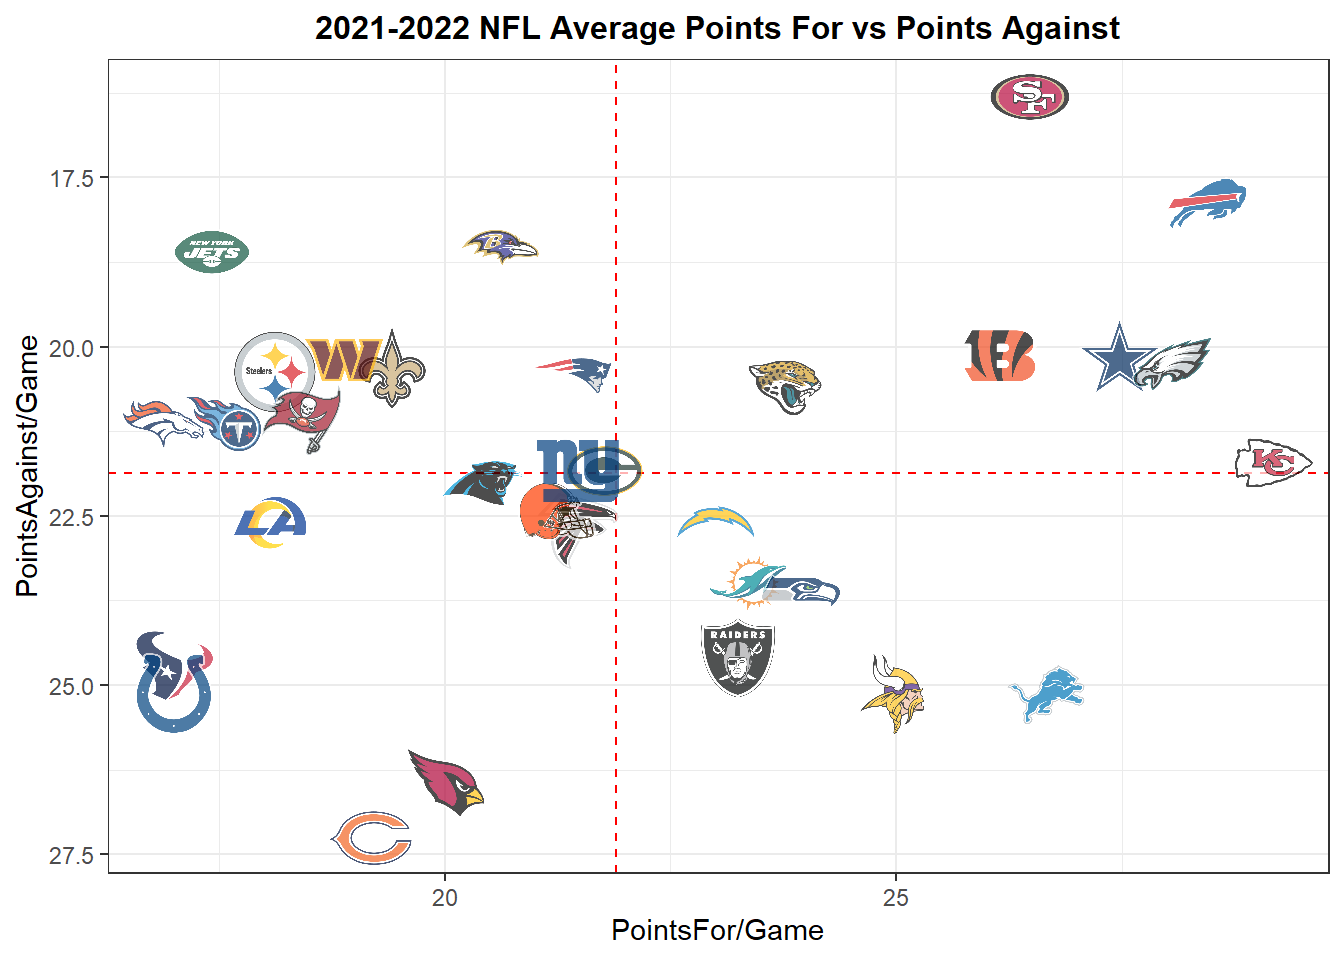
\includegraphics{_main_files/figure-latex/unnamed-chunk-2-1.pdf}

\begin{Shaded}
\begin{Highlighting}[]
\FunctionTok{ggplot}\NormalTok{(team\_df, }\FunctionTok{aes}\NormalTok{(}\AttributeTok{x =}\NormalTok{ pointsFor, }\AttributeTok{y =}\NormalTok{ netPF)) }\SpecialCharTok{+}
  \FunctionTok{geom\_mean\_lines}\NormalTok{(}\FunctionTok{aes}\NormalTok{(}\AttributeTok{h\_var =}\NormalTok{ pointsFor, }\AttributeTok{v\_var =}\NormalTok{ netPF)) }\SpecialCharTok{+}
  \FunctionTok{geom\_nfl\_logos}\NormalTok{(}\FunctionTok{aes}\NormalTok{(}\AttributeTok{team\_abbr =}\NormalTok{ team), }\AttributeTok{width =} \FloatTok{0.07}\NormalTok{, }\AttributeTok{alpha =} \FloatTok{0.7}\NormalTok{) }\SpecialCharTok{+}
  \FunctionTok{labs}\NormalTok{(}\AttributeTok{x =} \StringTok{"Actual Points For"}\NormalTok{,}
       \AttributeTok{y =} \StringTok{"Weighted Points For"}\NormalTok{,}
       \AttributeTok{title =} \StringTok{"2022{-}2023 NFL Points For vs Weighted Points For Based On Opponent"}\NormalTok{) }\SpecialCharTok{+}
  \FunctionTok{theme\_bw}\NormalTok{() }\SpecialCharTok{+}
  \FunctionTok{theme}\NormalTok{(}\AttributeTok{plot.title =} \FunctionTok{element\_text}\NormalTok{(}\AttributeTok{size =} \DecValTok{12}\NormalTok{, }\AttributeTok{hjust =} \FloatTok{0.5}\NormalTok{, }\AttributeTok{face =} \StringTok{"bold"}\NormalTok{))}
\end{Highlighting}
\end{Shaded}

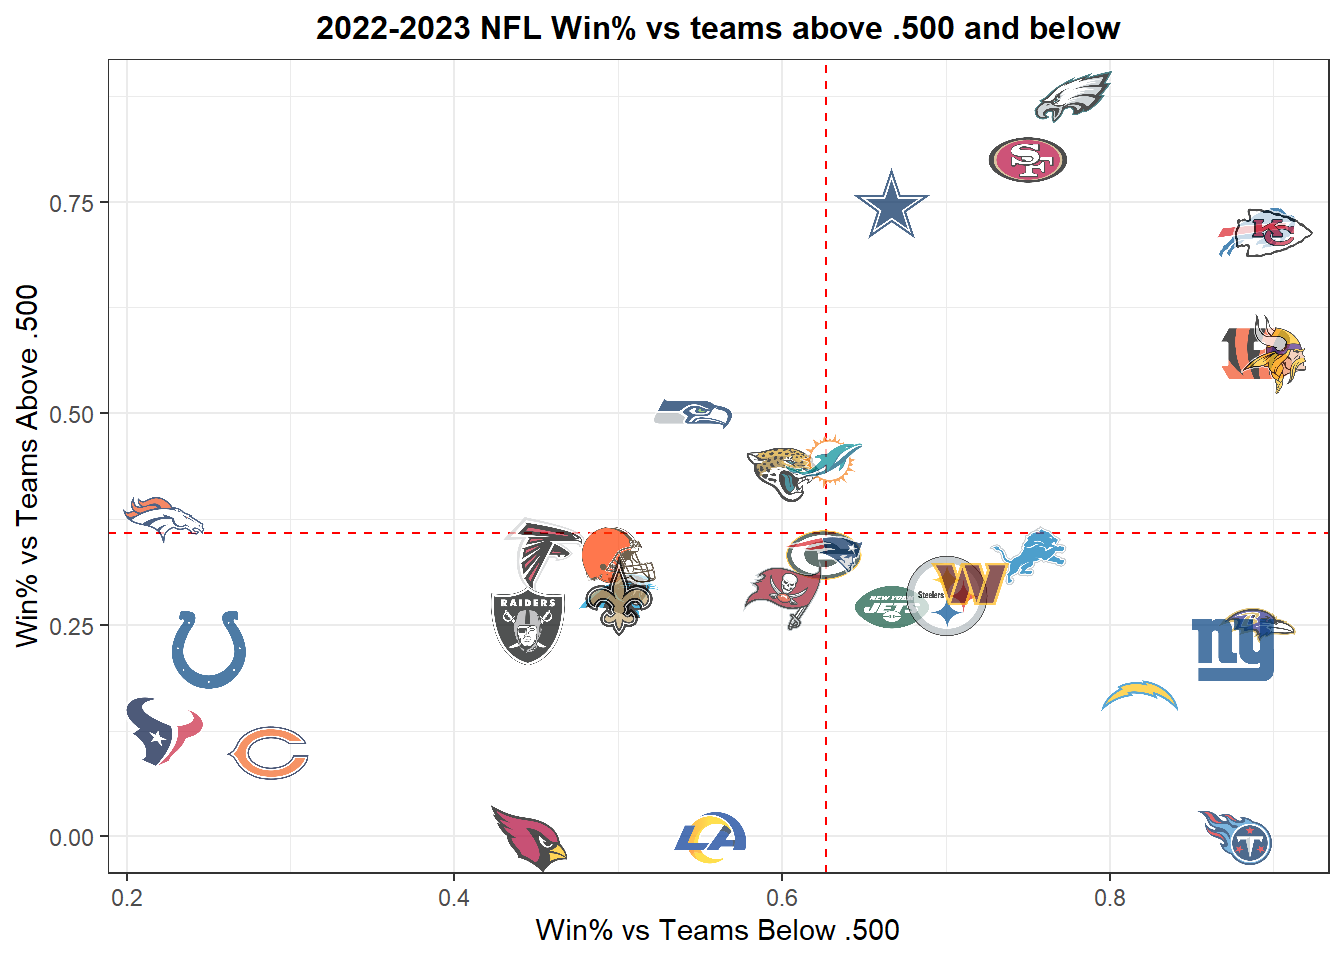
\includegraphics{_main_files/figure-latex/unnamed-chunk-3-1.pdf}

\begin{Shaded}
\begin{Highlighting}[]
\FunctionTok{ggplot}\NormalTok{(team\_df, }\FunctionTok{aes}\NormalTok{(}\AttributeTok{x =}\NormalTok{ pointsAgainst, }\AttributeTok{y =}\NormalTok{ netPA)) }\SpecialCharTok{+}
  \FunctionTok{geom\_mean\_lines}\NormalTok{(}\FunctionTok{aes}\NormalTok{(}\AttributeTok{h\_var =}\NormalTok{ pointsAgainst, }\AttributeTok{v\_var =}\NormalTok{ netPA)) }\SpecialCharTok{+}
  \FunctionTok{geom\_nfl\_logos}\NormalTok{(}\FunctionTok{aes}\NormalTok{(}\AttributeTok{team\_abbr =}\NormalTok{ team), }\AttributeTok{width =} \FloatTok{0.07}\NormalTok{, }\AttributeTok{alpha =} \FloatTok{0.7}\NormalTok{) }\SpecialCharTok{+}
  \FunctionTok{labs}\NormalTok{(}\AttributeTok{x =} \StringTok{"Actual Points Against"}\NormalTok{,}
       \AttributeTok{y =} \StringTok{"Weighted Points Against"}\NormalTok{,}
       \AttributeTok{title =} \StringTok{"2022{-}2023 NFL Points Against vs Weighted Points Against Based On Opponent"}\NormalTok{) }\SpecialCharTok{+}
  \FunctionTok{theme\_bw}\NormalTok{() }\SpecialCharTok{+}
  \FunctionTok{theme}\NormalTok{(}\AttributeTok{plot.title =} \FunctionTok{element\_text}\NormalTok{(}\AttributeTok{size =} \DecValTok{12}\NormalTok{, }\AttributeTok{hjust =} \FloatTok{0.5}\NormalTok{, }\AttributeTok{face =} \StringTok{"bold"}\NormalTok{))}\SpecialCharTok{+}
  \FunctionTok{scale\_y\_reverse}\NormalTok{()}\SpecialCharTok{+}
  \FunctionTok{scale\_x\_reverse}\NormalTok{()}
\end{Highlighting}
\end{Shaded}

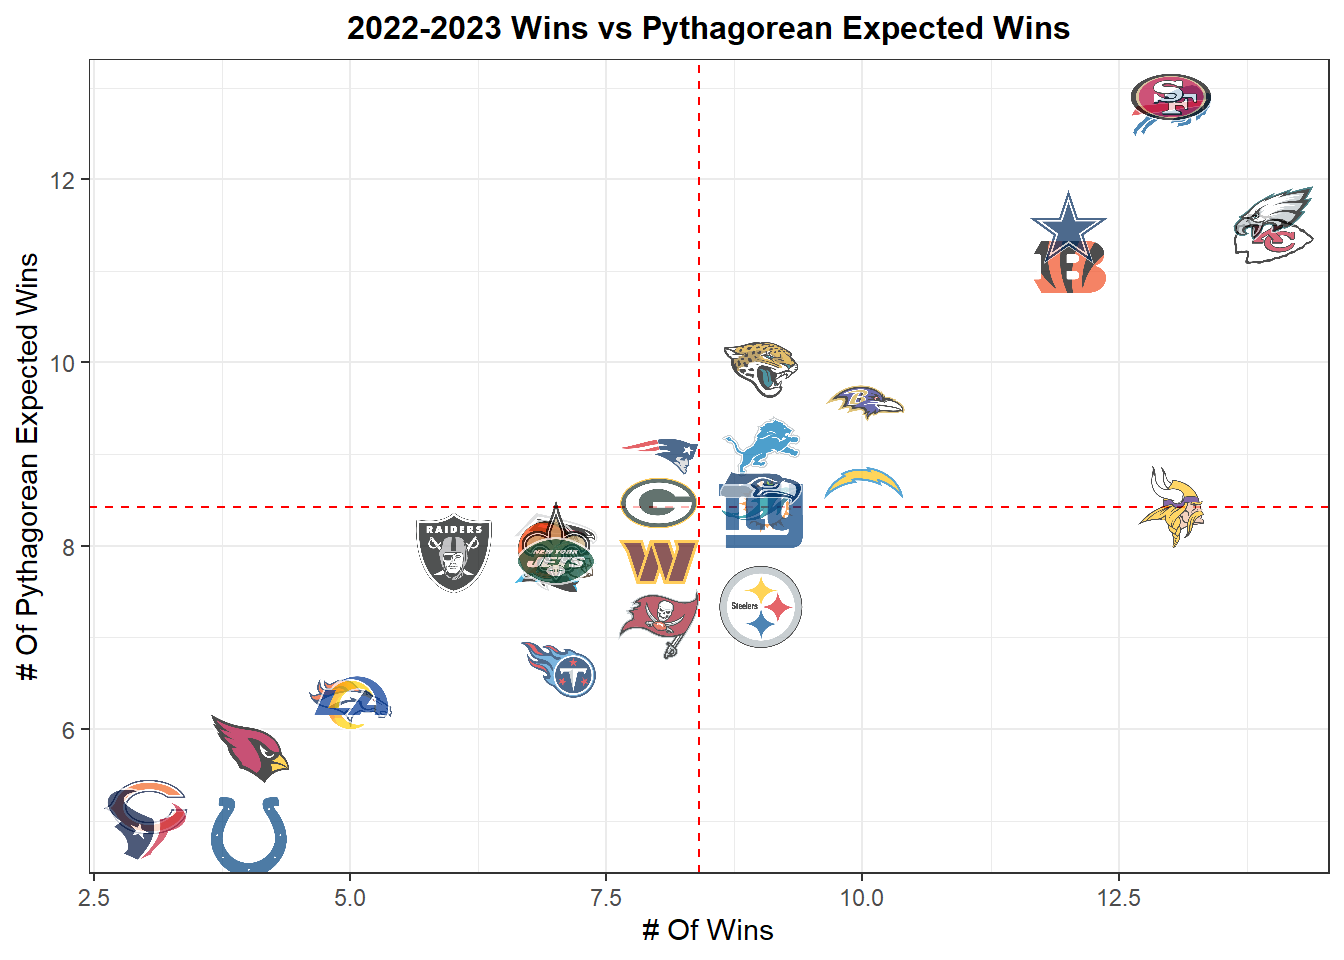
\includegraphics{_main_files/figure-latex/unnamed-chunk-4-1.pdf}

\hypertarget{game-props-predictions}{%
\subsection{Game Props Predictions}\label{game-props-predictions}}

\hypertarget{qb-data}{%
\section{QB Data}\label{qb-data}}

Here we will have all NFL QB-related Data and predictions

\hypertarget{general-data}{%
\subsection{General Data}\label{general-data}}

\begin{verbatim}
## `summarise()` has grouped output by 'passer'. You can override using the
## `.groups` argument.
## `summarise()` has grouped output by 'passer'. You can override using the
## `.groups` argument.
## `summarise()` has grouped output by 'passer'. You can override using the
## `.groups` argument.
## `summarise()` has grouped output by 'passer'. You can override using the
## `.groups` argument.
## `geom_smooth()` using formula = 'y ~ x'
\end{verbatim}

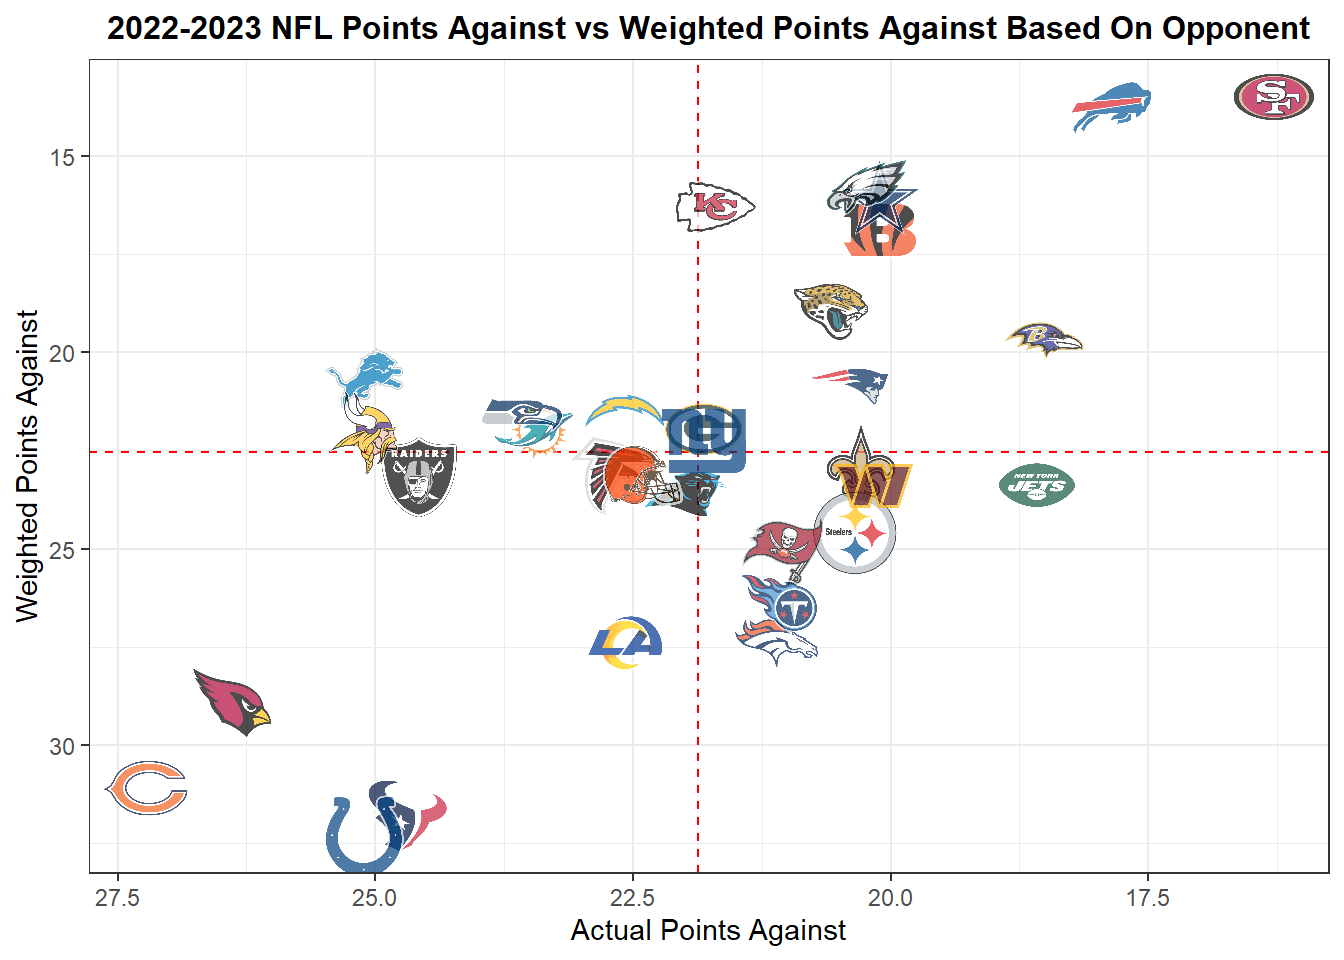
\includegraphics{_main_files/figure-latex/unnamed-chunk-6-1.pdf}

\begin{verbatim}
## `summarise()` has grouped output by 'passer'. You can override using the
## `.groups` argument.
## `summarise()` has grouped output by 'passer'. You can override using the
## `.groups` argument.
## `summarise()` has grouped output by 'passer'. You can override using the
## `.groups` argument.
## `summarise()` has grouped output by 'passer'. You can override using the
## `.groups` argument.
## `geom_smooth()` using formula = 'y ~ x'
\end{verbatim}

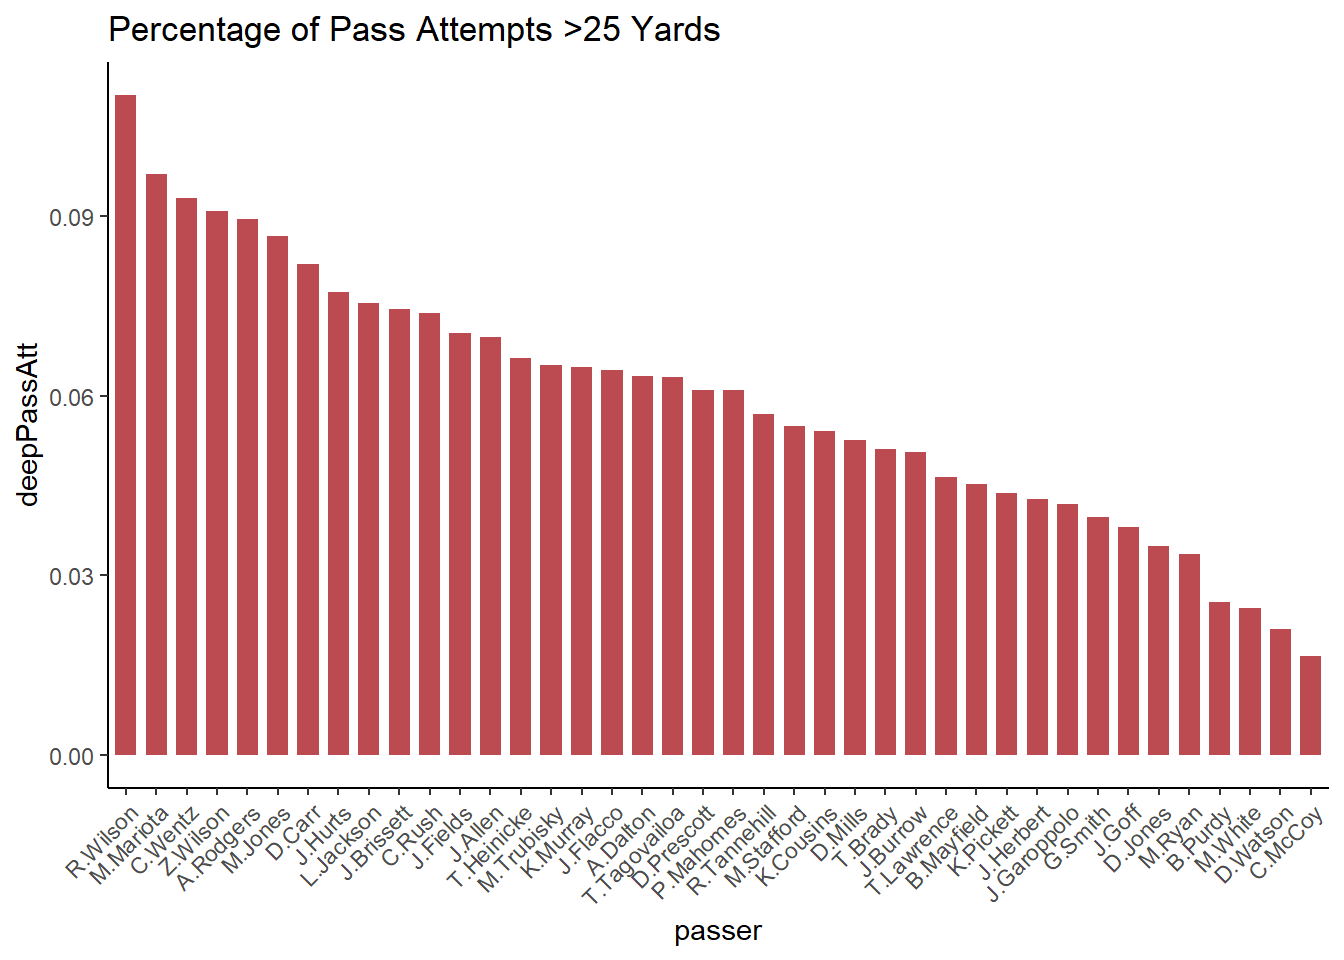
\includegraphics{_main_files/figure-latex/unnamed-chunk-7-1.pdf}

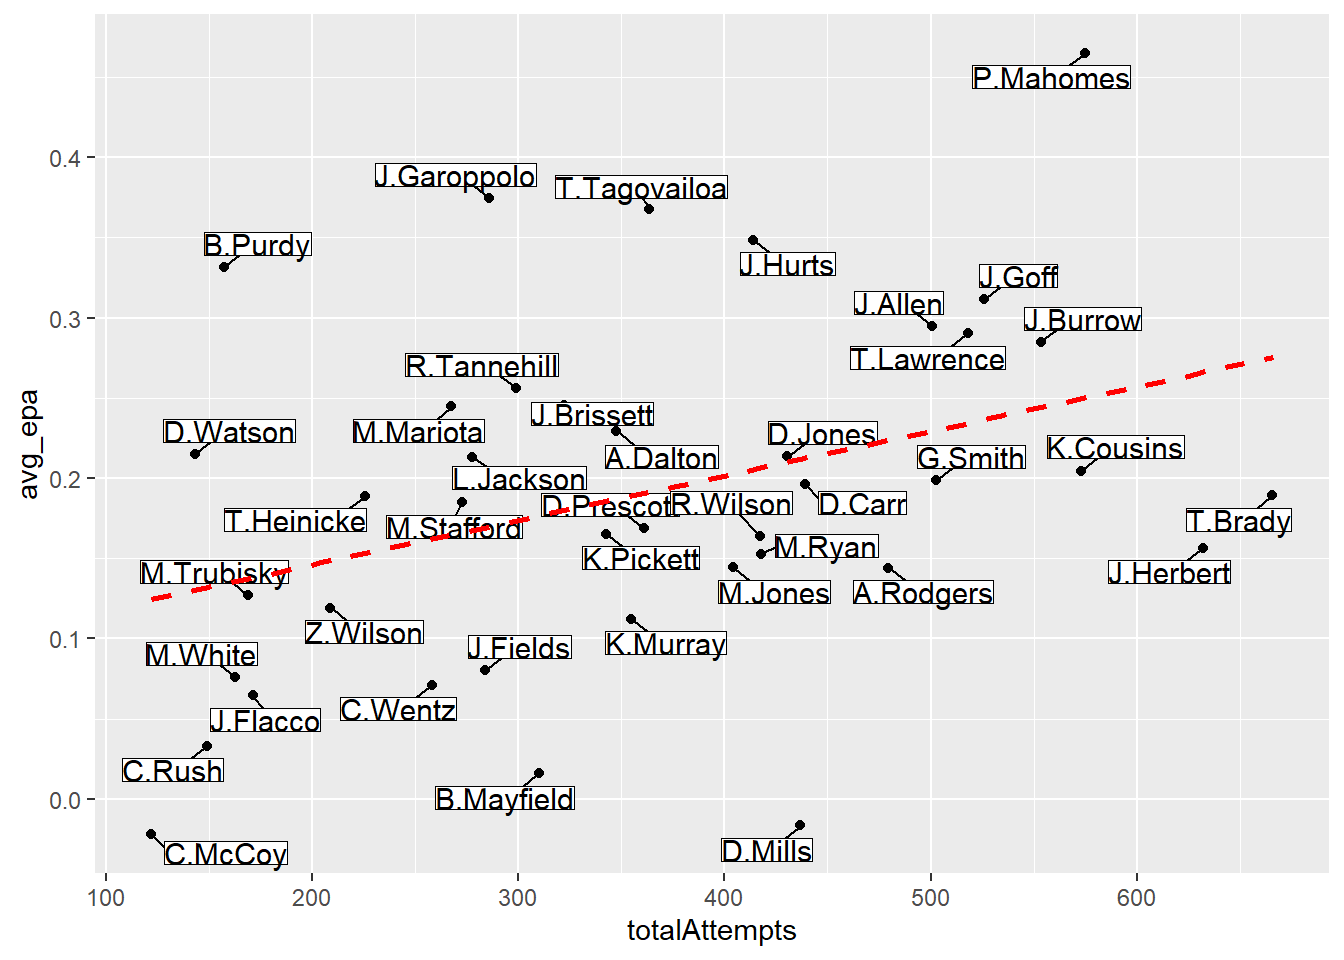
\includegraphics{_main_files/figure-latex/unnamed-chunk-8-1.pdf}

\begin{verbatim}
## `geom_smooth()` using formula = 'y ~ x'
\end{verbatim}

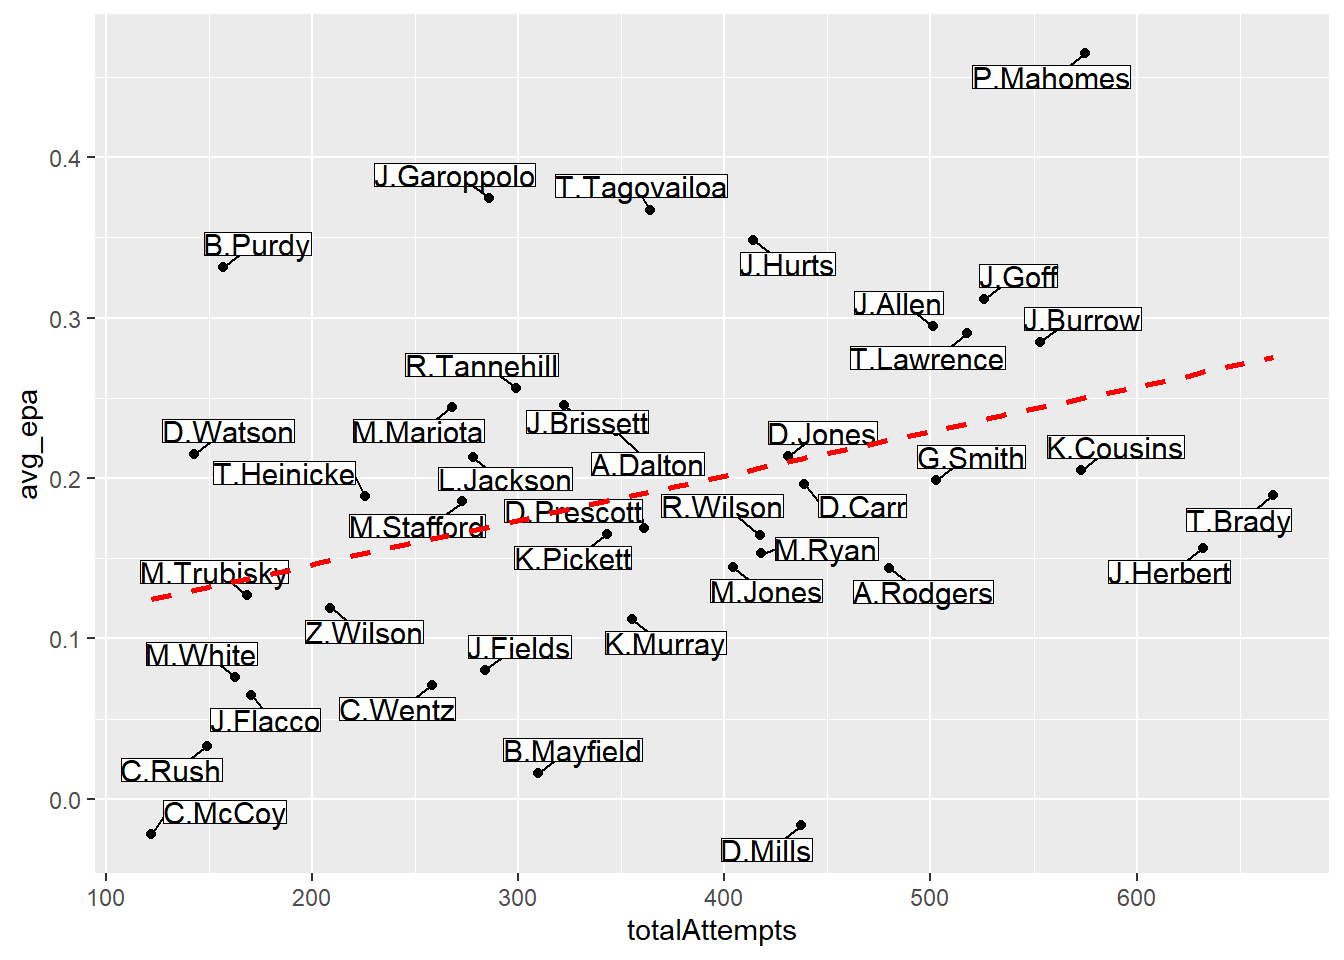
\includegraphics{_main_files/figure-latex/unnamed-chunk-9-1.pdf}

\begin{verbatim}
## `geom_smooth()` using formula = 'y ~ x'
\end{verbatim}

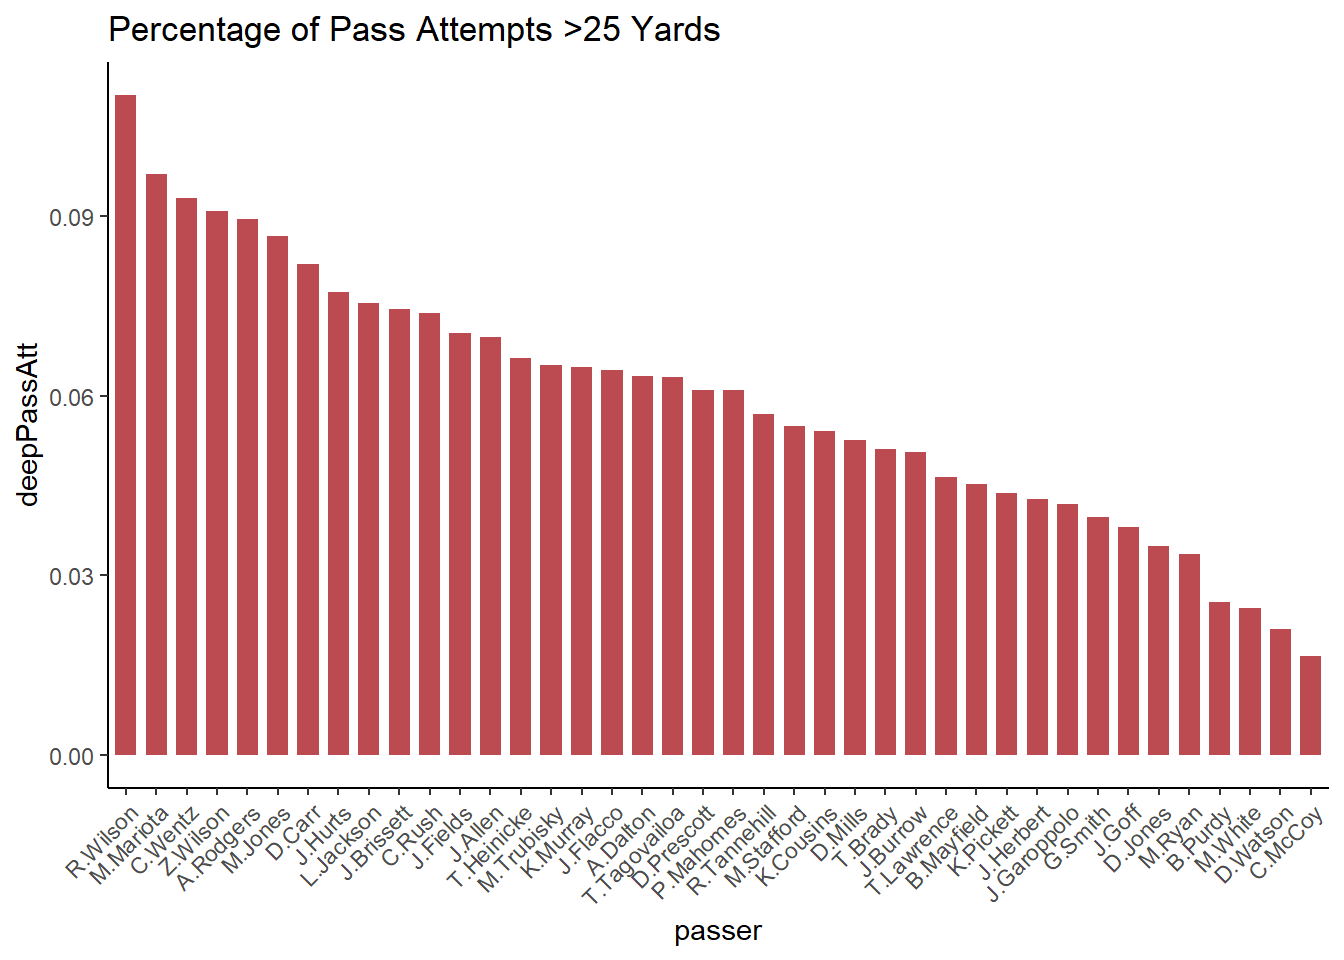
\includegraphics{_main_files/figure-latex/unnamed-chunk-10-1.pdf}

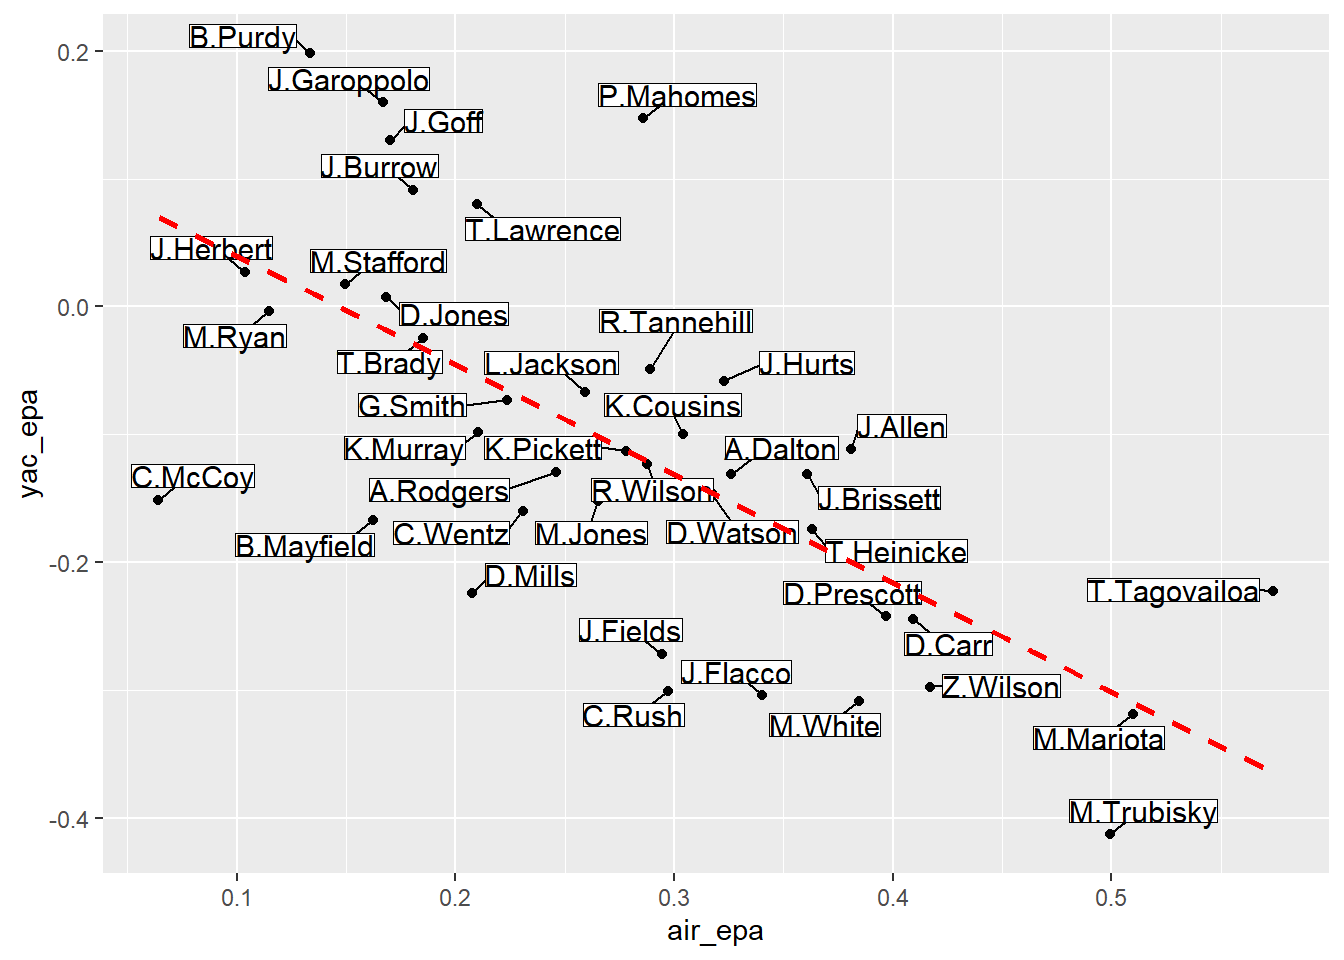
\includegraphics{_main_files/figure-latex/unnamed-chunk-11-1.pdf}

\begin{verbatim}
## `geom_smooth()` using formula = 'y ~ x'
\end{verbatim}

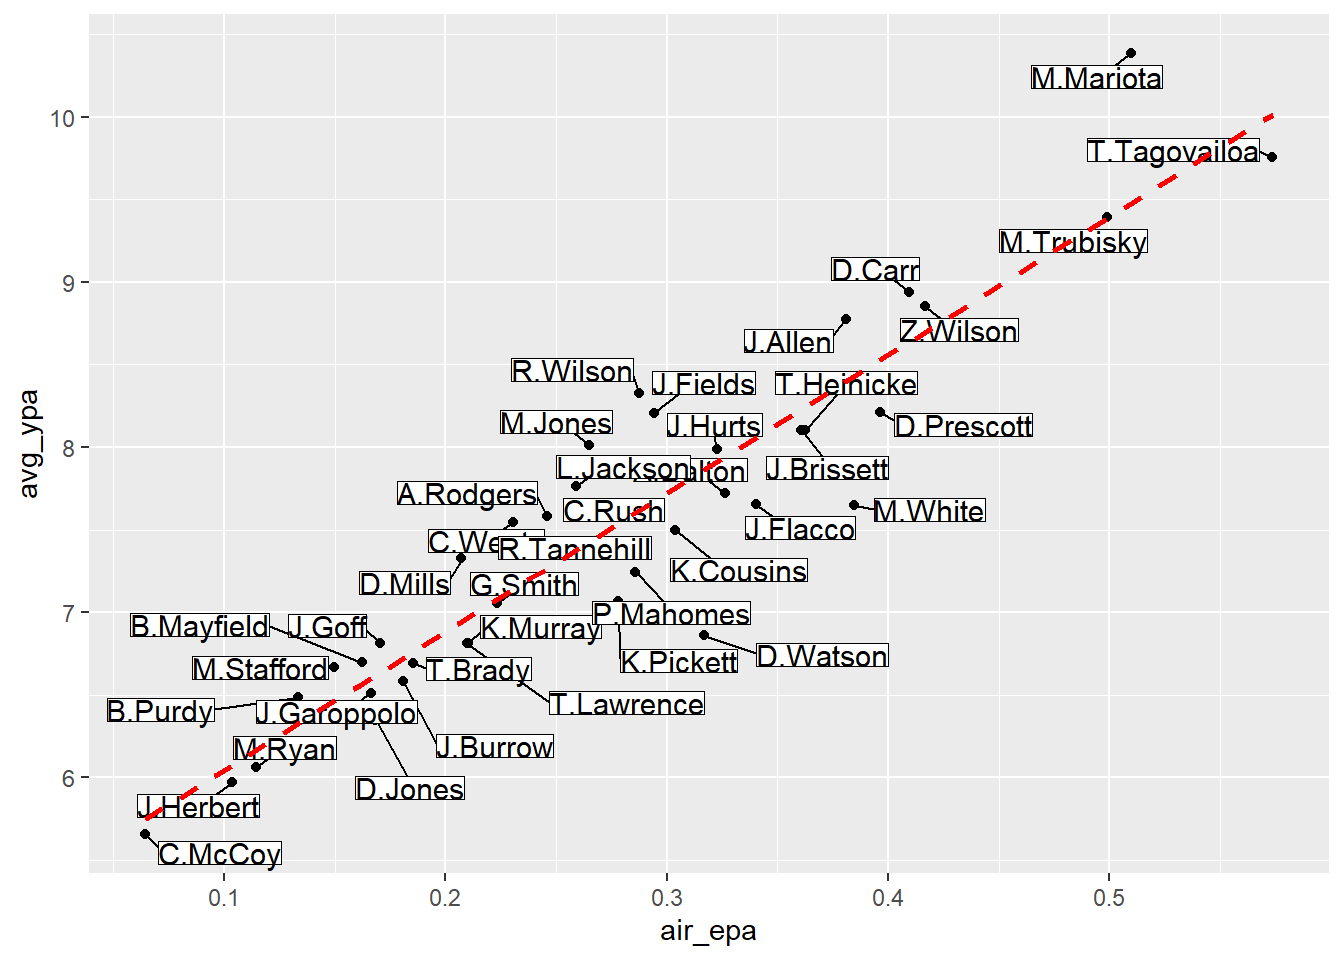
\includegraphics{_main_files/figure-latex/unnamed-chunk-12-1.pdf}

\begin{verbatim}
## `geom_smooth()` using formula = 'y ~ x'
\end{verbatim}

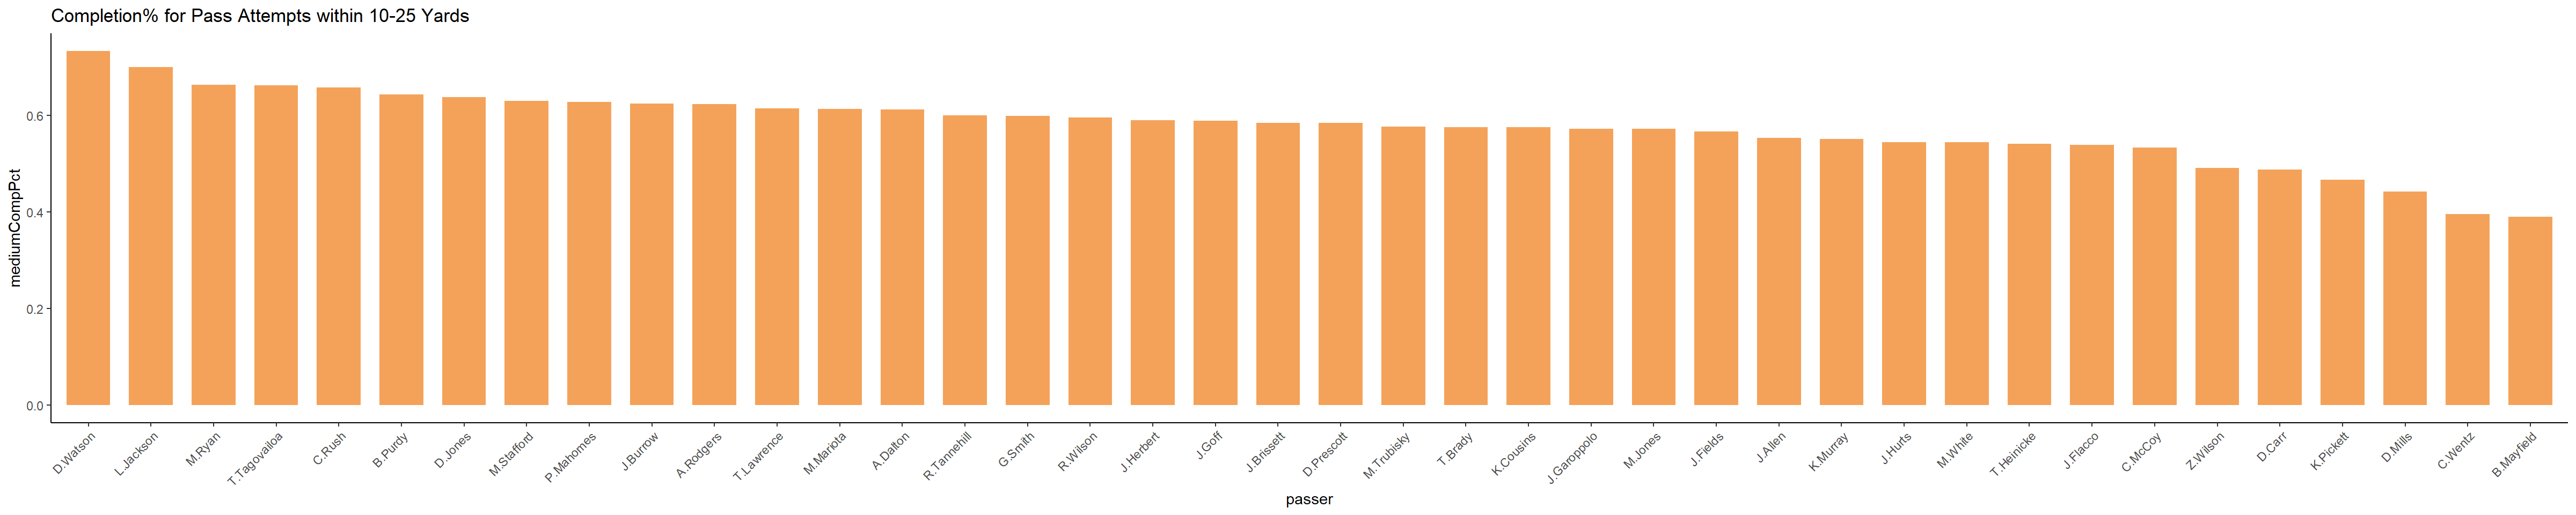
\includegraphics{_main_files/figure-latex/unnamed-chunk-12-2.pdf}

\begin{verbatim}
## `geom_smooth()` using formula = 'y ~ x'
\end{verbatim}

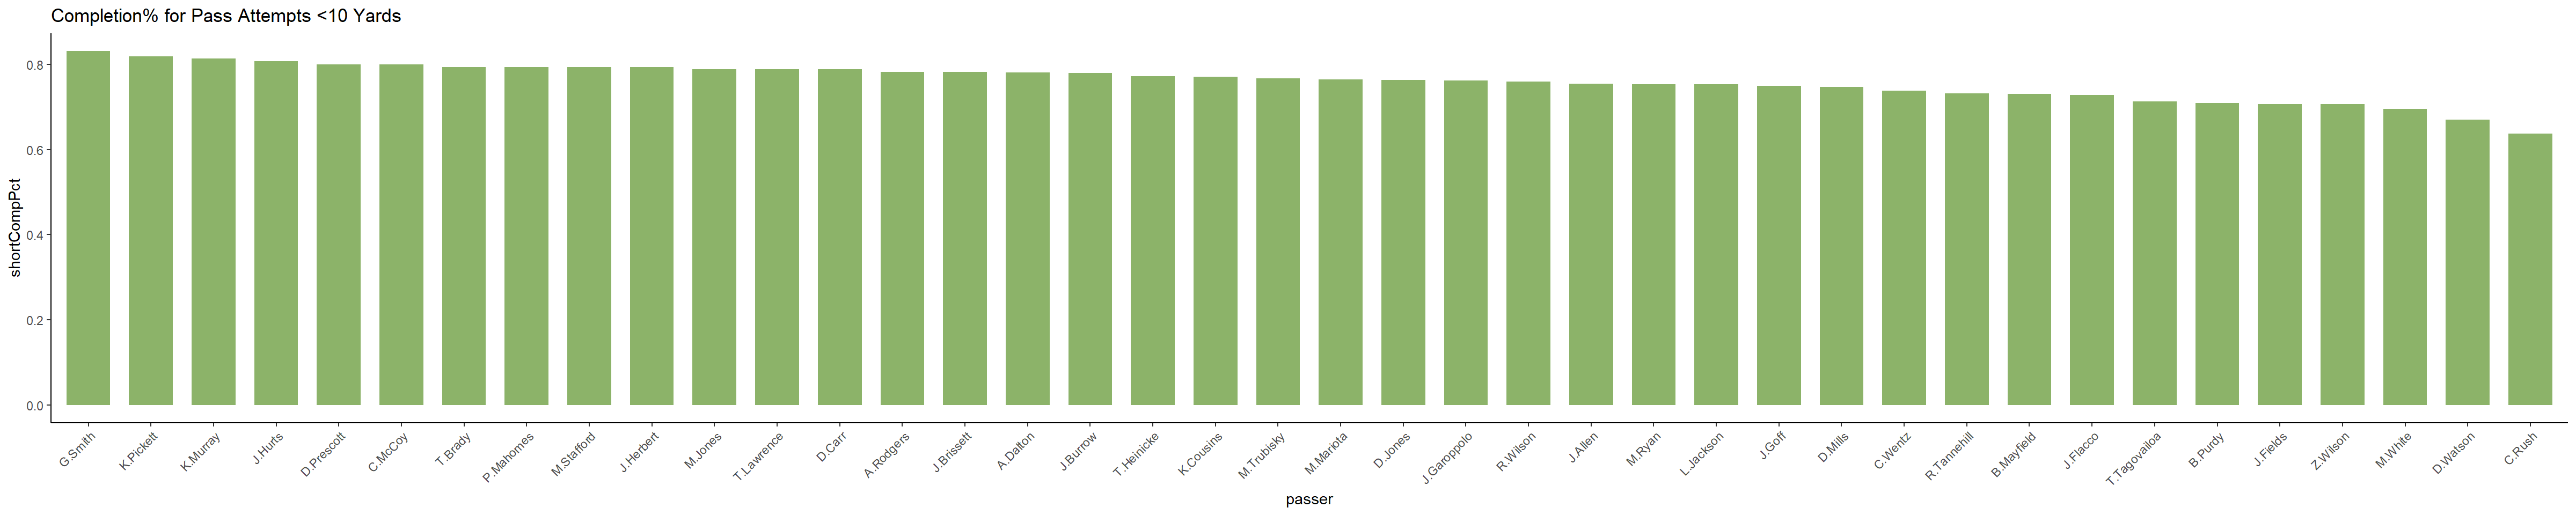
\includegraphics{_main_files/figure-latex/unnamed-chunk-12-3.pdf}

\end{document}
